\documentclass{report}
\usepackage{titling}
\usepackage{natbib} 
\usepackage{listings}
\usepackage{xcolor}
\usepackage{graphicx}
\usepackage{amsmath}
\usepackage{amssymb}
\usepackage{booktabs}
\usepackage[left=2cm,right=2cm,top=2cm,bottom=2cm]{geometry} 
\usepackage{multirow}
\usepackage{float}
\usepackage{tikz}
\usetikzlibrary{shapes,arrows,positioning,calc}


% Define colors for code highlighting
\definecolor{codegreen}{rgb}{0,0.6,0}
\definecolor{codegray}{rgb}{0.5,0.5,0.5}
\definecolor{codepurple}{rgb}{0.58,0,0.82}
\definecolor{backcolour}{rgb}{0.95,0.95,0.92}

% Define code listing style
\lstdefinestyle{mystyle}{
    backgroundcolor=\color{backcolour},   
    commentstyle=\color{codegreen},
    keywordstyle=\color{magenta},
    numberstyle=\tiny\color{codegray},
    stringstyle=\color{codepurple},
    basicstyle=\ttfamily\footnotesize,
    breakatwhitespace=false,         
    breaklines=true,                 
    captionpos=b,                    
    keepspaces=true,                 
    numbers=left,                    
    numbersep=5pt,                  
    showspaces=false,                
    showstringspaces=false,
    showtabs=false,                  
    tabsize=2
}
\newenvironment{highlights}{
    \begin{itemize}[
        topsep=0.10 cm,
        parsep=0.10 cm,
        partopsep=0pt,
        itemsep=0pt,
        leftmargin=0.4 cm + 10pt
    ]
}{
    \end{itemize}
} 
% Apply the custom code listing style
\lstset{style=mystyle}

% Define custom equation styles
\newcommand{\myeq}{\textcolor{blue}}
\centering
\title{Control Engineering Project}

\usepackage{caption}
\usepackage{tikz}
\usetikzlibrary{positioning, shapes.geometric, arrows.meta}

\usepackage{graphicx}
\usepackage{subcaption}
\usepackage[margin=1in]{geometry}

\begin{document}

\begin{titlepage}\begin{center}
    \begin{minipage}[c]{0.12\textwidth}
        
\includegraphics[width=\textwidth]{Cairo_University_Crest.png}
    \end{minipage}
    \hfill
    \begin{minipage}[c]{0.5\textwidth}
        \centering
        {\large Cairo University - Faculty Of Engineering \\ Computer Engineering Department \\ Control Engineering - Spring 2025 \par}
    \end{minipage}
    \hfill
    \begin{minipage}[c]{0.15\textwidth}
        
\includegraphics[width=\textwidth]{CUFE.jpeg}
    \end{minipage}
\end{center}

    \noindent\hrulefill
    
    \vspace*{2cm}
    {\LARGE \textbf{\ Two-Ttank System} \par}
    \vspace{1cm}

    
    \begin{center}
        \begin{tabular}{@{}||c||c||@{}}
            \toprule
            \Large \textbf{Name} & \Large \textbf{ID} \\ 
            \midrule 
            \multirow{2}{*}{\Large Ahmed Hamdy} & \multirow{2}{*}{\large 9220032} \\
                                                &                               \\
            \midrule 
            \multirow{2}{*}{\Large Abd El-Rahman Mostafa}  & \multirow{2}{*}{\large 9220475} \\
                                                &  \\
            \midrule
            \multirow{2}{*}{\Large Mohammed Khater}  & \multirow{2}{*}{\large 9220713} \\
                                                &                               \\
            \bottomrule
        \end{tabular}
    \end{center}
    \vspace{1.5cm}
    {\Large \textbf{Delivered to} \\ \vspace{0.25cm}
    Prof. Ragia Badr \\ \vspace{0.25cm}
    Dr. Meena Elia\\ \vspace{0.25cm}
    Eng. Hassan El-Menier
    
    \vfill
\end{titlepage}

\begin{flushleft}

\section*{Part 1: Dynamic Equations and Block Diagram}

\begin{figure}[H]
    \centering
    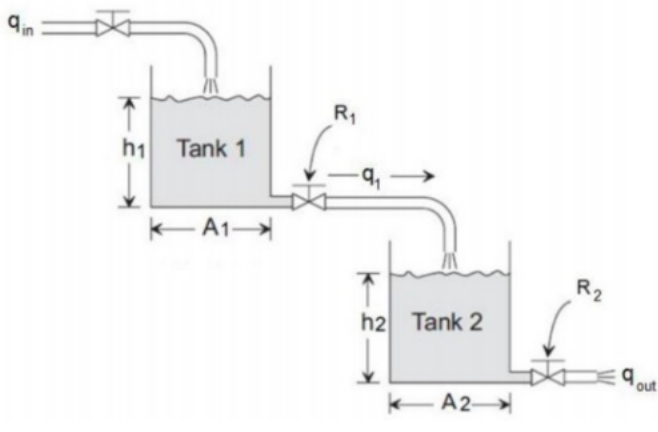
\includegraphics[width=0.5\linewidth]{system.png}
    \caption{Two-tank System}
    \label{fig:system}
\end{figure}

\subsection*{Dynamic Equations}
For Tank 1:

\begin{align}
    q_{\text{in}}(t) - q_{1}(t) &= A_1 \frac{dh_1}{dt}
    \quad \longrightarrow\quad Q_{\text{in}}(S) - Q_{1}(S) = A_1 SH_{1}(S) 
    \label{eq:tank1_balance}
\end{align}

\begin{align}
    q_{1}(t) &= \frac{h_1(t) - h_2(t)}{R_1}
        \quad \longrightarrow \quad  Q_{\text{1}}(S) = \frac{H_{1}(S) - H_{2}(S)}{R_{1}}
    \label{eq:tank1_flow}
\end{align}

Substituting \eqref{eq:tank1_flow} into \eqref{eq:tank1_balance}:
\begin{align}
    \frac{dh_1}{dt} &= \frac{1}{A_1} \left( q_{\text{in}}(t) - \frac{h_1(t) - h_2(t)}{R_1} \right)
     \quad \longrightarrow \quad  H_{\text{1}}(S) = \frac{1}{SA_{1}}\left( Q_{in}(S) - \frac{H_{1}(S) - H_{2}(S)}{R_{1}}\right)
    \label{eq:tank1_final}
\end{align}

For Tank 2:

\begin{align}
    q_{\text{1}}(t) - q_{2}(t) &= A_2 \frac{dh_2}{dt} \quad \longrightarrow\quad Q_{\text{1}}(S) - Q_{2}(S) = A_2 SH_{2}(S)
    \label{eq:tank2_balance}
\end{align}

Output flow:
\begin{align}
    q_{2}(t) &= \frac{h_2(t)}{R_2}\quad \longrightarrow \quad  Q_{\text{2}}(S) = \frac{H_{2}(S)}{R_{2}}
    \label{eq:tank2_flow}
\end{align}

Substituting \eqref{eq:tank2_flow} into \eqref{eq:tank2_balance}:

\begin{align}
    \frac{dh_2}{dt} &= \frac{1}{A_2} \left( \frac{h_1(t) - h_2(t)}{R_1} - \frac{h_2(t)}{R_2} \right)\quad \longrightarrow \quad  H_{\text{2}}(S) = \frac{1}{SA_{2}}\left( \frac{H_{1}(S) - H_{2}(S)}{R_{2}} - \frac{H_{2}(S)}{R_{2}}\right)
    \label{eq:tank2_final}
\end{align}



\newpage
\begin{align*}
& Q_2(S) = Q_{in}(S) - A_1 S H_1(S) - A_2 S H_2(S) \\
\\&Q_2(S) = Q_{in}(S) - A_1 S [Q_1(S)R_1 + H_2(S)] - A_2 S [R_2 Q_2(S)] \\
\\&Q_2(S) = Q_{in}(S) - A_1 S Q_2(S) R_1 - A_1 A_2 S^2 H_2(S) R_1 - A_1 S R_2 Q_2(S) - A_2 S R_2 Q_2(S) \\
\\&Q_2(S) = Q_{in}(S) - A_1 S Q_2(S) R_1 - A_1 A_2 S^2 [R_1 Q_2(S)] R_1 - A_1 S R_2 Q_2(S) - A_2 S R_2 Q_2(S) \\
\\&Q_2(S)\big[1 + A_1 S R_1 + A_1 A_2 S^2 R_1 R_2 + A_1 S R_2 + A_2 S R_2\big] = Q_{in}(S) \\
\end{align*}

\subsection*{Block Diagram Representation}
\begin{figure}[h]
\centering
\begin{tikzpicture}[auto, node distance=2cm, >=latex']

% Define block styles
\tikzstyle{block} = [draw, rectangle, minimum height=2em, minimum width=4em]
\tikzstyle{sum} = [draw, circle, inner sep=0pt, minimum size=5mm]
\tikzstyle{input} = [coordinate]
\tikzstyle{output} = [coordinate]
\tikzstyle{pinstyle} = [pin edge={to-,thin,black}]

% Nodes
\node [input, name=input] {};
\node [sum, right of=input] (sum1) {$+$};
\node [output, right of=sum1] (blck){};
\node [block, right of=blck] (int1) {$\dfrac{1}{A_1S}$};
\node [output, right of=int1] (output1) {};
\node [block, below of=int1] (feedback1) {$\dfrac{1}{A_2S}$};
\node [sum, left of=feedback1] (sum3) {$+$};
\node [output, left of=sum3] (output12){};
\node [sum, right of=output1] (sum2) {$+$};
\node [output, below of=sum2]  (output2){};
\node [output, below of=output2]  (output3){};
\node [block, below of=feedback1] (feedback2) {$\dfrac{1}{R_2}$};
\node [output, below of=output2]  (output3){};
\node [block, below of=feedback2] (feedback3) {$\dfrac{1}{R_1}$};
\node [output, right of=sum2] (output4){};
\node [output, right of=feedback3] (output5){};
\node [output, right of=output5] (output6){};
\node [output, right of=output6] (output7){};
\node [output, left of=feedback3] (output8){};
\node [output, left of=output8] (output9){};
\node [output, left of=feedback2] (output10){};

% Connections
\draw [->] (input) -- node[pos=0.9] {$+$} node {$Q_{in}(S)$} (sum1);
\draw [->] (sum1) -- node {} (int1);
\draw [->] (int1) -- node[name=h1] {$H_1(S)$} node [pos=0.9] {$+$} (sum2);
\draw [<-] (sum2) |- node[pos=0.8] {$H_2(S)$} node [pos=0.1] {$-$} (feedback1);
\draw [->] (blck) -- node[pos=0.9] {$-$} (sum1);
\draw [-] node {} (output2) --  (output3);
\draw [->] node {} (output3) --  (feedback2);
\draw [-] (sum2) --  (output4);
\draw [-] (output4) --  (output7);
\draw [->] (output7) --  (feedback3);
\draw [-] (feedback3) --  (output9);
\draw [->] (output9) --  (sum1);
\draw [->] (sum3) --  (feedback1);
\draw [->] (output12) -- node[pos=0.9] {$+$} node {$Q_{1}(S)$} (sum3);
\draw [-] (feedback2) -- node[pos=0.5] {$Q_2(S)$} (output10);
\draw [->] (output10) --  node[pos=0.9] {$-$} (sum3);

\end{tikzpicture}
\caption{Block diagram of the system}
\label{fig:unsimplified_block_diagram}
\end{figure} 

\newpage
\section*{Simulation}
\subsubsection*{Obtaining Transfer Functions using MATLAB}

\large{System Parameters:}$\quad\quad A_1 = 5m^2,\quad A_2 = 4m^2,\quad R_1 = 3 s/m^2,\quad R_2 = 5 s/m^2$

Using Matlab, we get the following results:
\begin{align*}
 &\frac{H_2(S)}{Q_{in}(S)} = \frac{5}{300 S^2 + 60S + 1}\\
\\&\frac{H_1(S)}{Q_{in}(S)} = \frac{60S+8}{300 S^2 + 60S + 1}\\
\\ &\frac{Q_1(S)}{Q_{in}(S)} = \frac{20S+1}{300 S^2 + 60S + 1} \\ 
\\&\frac{Q_2(S)}{Q_{in}(S)} = \frac{1}{300 S^2 + 60S + 1}\\
\end{align*}

\begin{figure}[H]
    \centering
    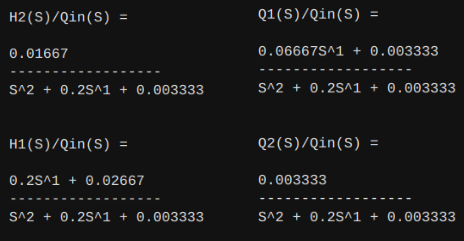
\includegraphics[width=0.7\linewidth]{tfs.png}
    \caption{Transfer Functions}
    \label{fig:tfs}
\end{figure}
\newpage 
\subsection*{Studying Stability}
Studying the stability of the system by analyzing the denominator of TF:
$
300 S^2 + 60S + 1=0$\\
We find that the system has 2 poles:\\
\[ P_{0} = -0.18165, \quad P_{1} = -0.01835 \]
\\ We can see that both of them lie on the left half of the plane, which means that the system is stable. We also
checked it using the isstable() function in MATLAB.
\begin{figure}[H]
    \centering
    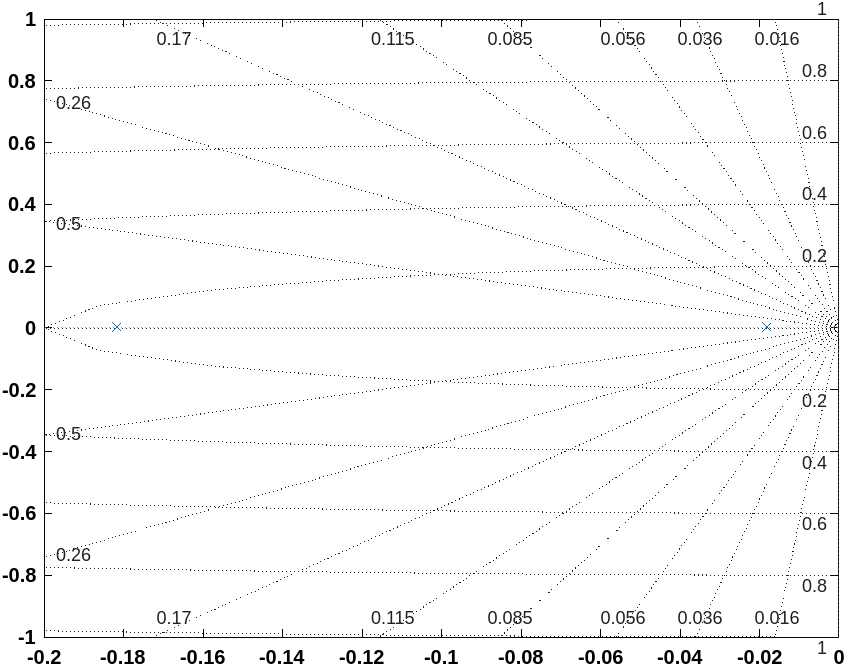
\includegraphics[width=0.75\linewidth]{system-poles.png}
    \caption{Pole-Zero map of the system}
    \label{fig:system poles}
\end{figure}
\end{flushleft}
\newpage
\begin{flushleft}
\subsection*{Simulating with $Q_{in}=1m/s$}

After simulating we get the following results

\begin{figure}[H]
    \centering
    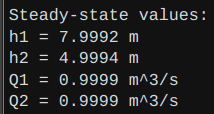
\includegraphics[width=0.4\linewidth]{req4-sol.png}
    \caption{Steady State Values for System Outputs}
    \label{fig:req-4}
\end{figure}


\begin{figure}[H]
    \centering
    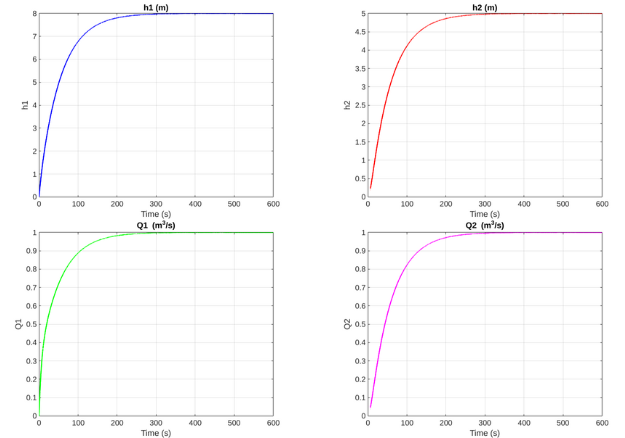
\includegraphics[width=0.8\linewidth]{rwq44.png}
    \caption{Time Responses for System Outputs}
    \label{fig:req-4}
\end{figure}
\textbf{Theoretically}
\[
h_1(t\approx \infty) = \lim_{S\to0} SH_1(S) \approx 8\;m 
\]
\[
h_2(t\approx \infty) = \lim_{S\to0} SH_2(S) \approx 5\; m 
\]\[
q_1(t\approx \infty) = \lim_{S\to0} SQ_1(S) \approx 1\;m^3/s 
\]
\[
q_2(t\approx \infty) = \lim_{S\to0} SQ_2(S) \approx 1\;m^3/s
\]


\end{flushleft}

\newpage
\begin{flushleft}
\section*{Part 2: Feedback Modification and Stability Check}
\subsection* {Representation of the feedback modification block diagram}
\begin{figure}[h]
\centering
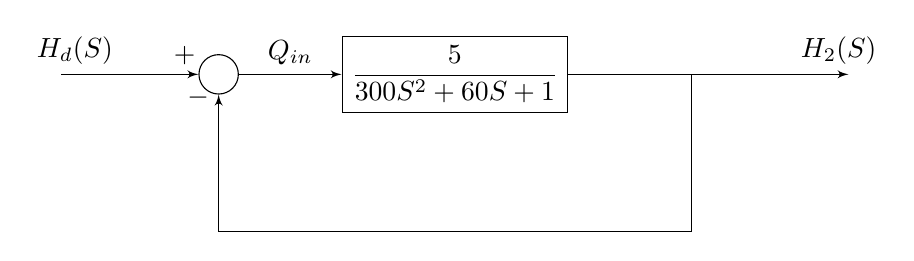
\begin{tikzpicture}[auto, node distance=2cm, >=latex']

% Define block styles
\tikzstyle{block} = [draw, rectangle, minimum height=2em, minimum width=4em]
\tikzstyle{sum} = [draw, circle, inner sep=0pt, minimum size=5mm]
\tikzstyle{input} = [coordinate]
\tikzstyle{output} = [coordinate]
\tikzstyle{pinstyle} = [pin edge={to-,thin,black}]

% Nodes
\node [input, name=input] {};
\node [sum, right of=input] (sum1) {};
\node [block, right of=sum1, node distance=3cm] (int1) {$\dfrac{5}{300S^2 + 60S + 1}$}; % Increased distance
\node [coordinate, right of=int1, node distance=3cm] (feedback) {}; % Point for feedback
\node [output, right of=feedback, node distance=2cm] (output) {}; % Extended output

% Connections
\draw [->] (input) -- node[pos=0.9, above] {$+$} node[pos=0.1, above] {$H_d(S)$} (sum1); % Input H_d to summer with + sign
\draw [->] (sum1) -- node[pos=0.5, above] {$Q_{in}$} (int1); % Summer to block with Q_in label
\draw [-] (int1) -- node[pos=2.2,above] {$H_2(S)$} (feedback); % Block to feedback point
\draw [->] (feedback) -- (output); % Feedback point to extended output
\draw [->] (feedback) |- ++(0,-2cm) -| node[pos=0.99, left] {$-$} (sum1); % Unity feedback with - sign beside

\end{tikzpicture}
\caption{Block Diagram of the Feedback-Modified System}
\label{fig:feedback_block_diagram}
\end{figure}

\subsection*{Simulating with $h_{d}=5 m $}
After simulating we get the following results

\begin{figure}[H]
    \centering
    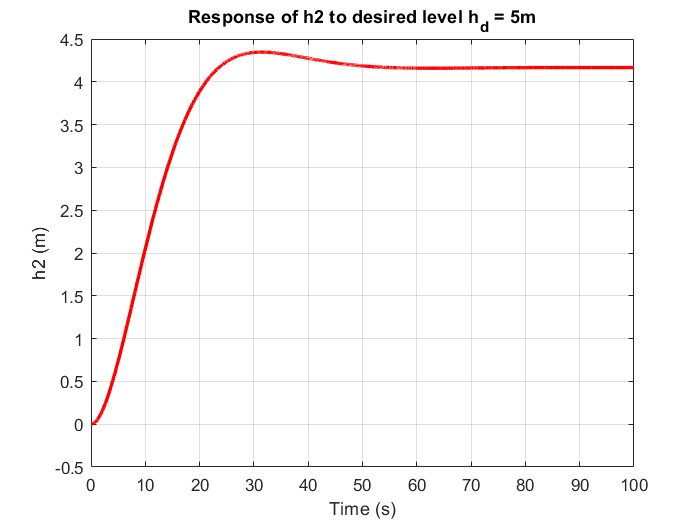
\includegraphics[width=0.4\linewidth]{feedback.png}
    \caption{Steady-State Response for Feedback Stabilization}
    \label{fig:req-5}
\end{figure}


\newpage
\centering
\textbf{Theoretically}
\\
% System parameters
\begin{description}
\item[Natural frequency] 
\[
\omega_n^2 = \dfrac{1}{50} \implies \omega_n = \dfrac{1}{5\sqrt{2}}
\]
\item[Damping ratio] 
\[
2\zeta\omega_n = \dfrac{1}{5} \implies \zeta = \dfrac{1}{\sqrt{2}}
\]
\item[Phase angle] 
\[
\zeta = \cos\psi = \dfrac{1}{\sqrt{2}} \implies \psi = \dfrac{\pi}{4}
\]
\item[Steady-state gain] 
\[
M = \lim_{s \to 0} s H_2(s) = \dfrac{5}{6}h_d \approx 4.1667
\]
\item[Resonant frequency] 
\[
\omega = \omega_n \sin\psi = \dfrac{1}{10}
\]
\item[Rise time] 
\[
t_r = \dfrac{\pi - \psi}{\omega} = \dfrac{15}{2}\pi \approx 23.562 \, \text{seconds}
\]
\item[Peak time] 
\[
t_p = \dfrac{\pi}{\omega} = 10\pi \approx 31.416 \, \text{seconds}
\]
\item[Peak overshoot] 
\[
M_p = M \left(1 + e^{-\dfrac{\pi}{\tan\psi}}\right) = M \left(1 + e^{-\pi}\right) \approx 4.3467 \, \text{meters}
\]
\item[Settling time] 
\[
t_s = \dfrac{4}{\zeta\omega_n} = 40 \, \text{seconds} \quad (\text{2\% criterion})
\]
\item[Steady-state error] 
\[
e_{ss} = 5 - 4.1667 = 0.8333 \, \text{meters}
\]
\end{description}

\newpage
\section*{adding a proportional controller}
\begin{figure}[H]
\centering

% TikZ diagram
\tikzset{
  block/.style = {draw, rectangle, minimum height=2em, minimum width=4em},
  input/.style = {coordinate},
  output/.style = {coordinate},
  sum/.style = {draw, circle, inner sep=0mm, minimum size=5mm},
  arrow/.style = {->, >=stealth},
}

\begin{tikzpicture}[auto, node distance=2cm,>=latex']
  \node [input] (input) {};
  \node [sum, right of=input] (sum) {};
  \node [block, right of=sum, node distance=2.5cm] (kp) {$K_p$};
  \node [block, right of=kp, node distance=3.2cm] (plant) {$\frac{5}{300s^2 + 60s + 1}$};
  \node [output, right of=plant, node distance=3.5cm] (output) {};
  \node [coordinate, below of=plant] (feedback) {};

  \draw [arrow] (input) -- node {$H_d(s)$} (sum);
  \draw [arrow] (sum) -- node {$Q_{in}$} (kp);
  \draw [arrow] (kp) -- (plant);
  \draw [arrow] (plant) -- node {$H_2(s)$} (output);
  \draw [arrow] (output) |- (feedback) -| node[pos=0.95] {$-$} (sum);
\end{tikzpicture}

\vspace{0.5em}
\caption{Block diagram of a unity feedback control system with a proportional controller \(K_p\).}

\vspace{1.5em}

% Image rows
\begin{subfigure}[b]{0.45\textwidth}
    \centering
    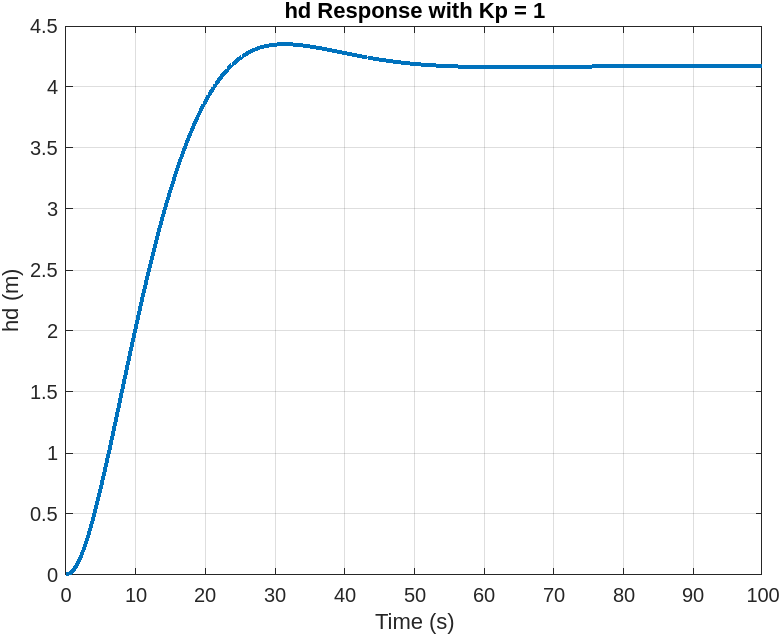
\includegraphics[width=\textwidth]{kpequals1.png}
    \caption{Figure 9: proportional controller with kp = 1}
\end{subfigure}
\hfill
\begin{subfigure}[b]{0.45\textwidth}
    \centering
    \includegraphics[width=\textwidth]{kpequal1Simulated.png}
    \caption{Figure 10: Transient Response Output with kp = 1}
\end{subfigure}

\vspace{1em}

\begin{subfigure}[b]{0.45\textwidth}
    \centering
    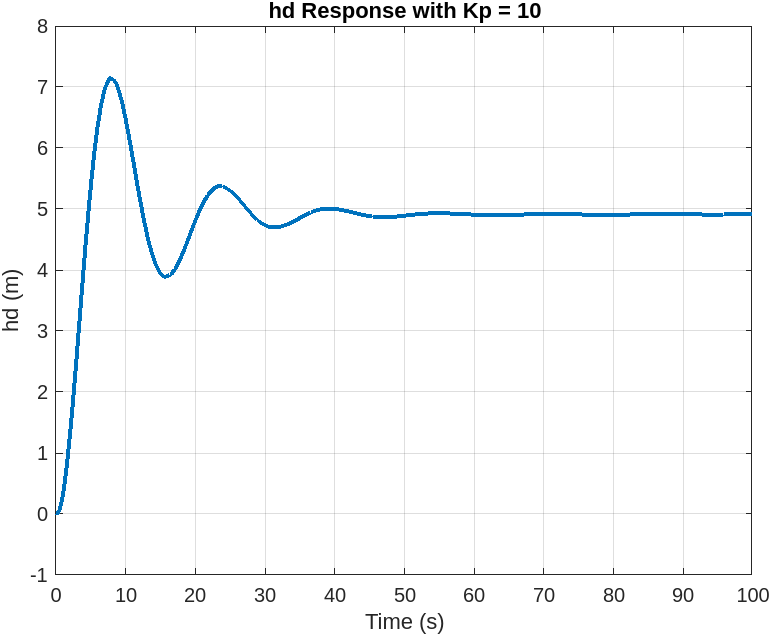
\includegraphics[width=\textwidth]{kqequals10.png}
    \caption{Figure 11: proportional controller with kp = 10}
\end{subfigure}
\hfill
\begin{subfigure}[b]{0.45\textwidth}
    \centering
    \includegraphics[width=\textwidth]{10.png}
    \caption{Figure 12: Transient Response Output with kp = 10}
\end{subfigure}

\vspace{1em}

\begin{subfigure}[b]{0.45\textwidth}
    \centering
    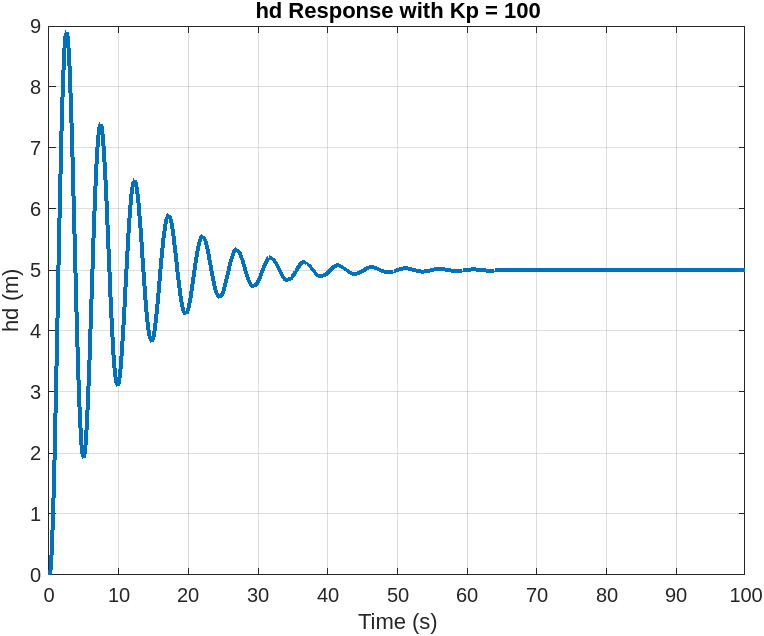
\includegraphics[width=\textwidth]{kpequals100.png}
    \caption{Figure 13: proportional controller with kp = 100}
\end{subfigure}
\hfill
\begin{subfigure}[b]{0.45\textwidth}
    \centering
    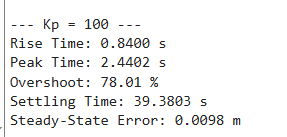
\includegraphics[width=\textwidth]{100.png}
    \caption{Transient Response Output with kp = 100}
\end{subfigure}

\caption*{Figure 14: Simulated responses for varying \(K_p\) values.}

\end{figure}

\newpage
\section*{Comment on Previous Results}
Increasing \( K_p \) decreases the steady-state error (ESS), but also reduces the system's stability and increases the transient response parameters.

\noindent\rule{\linewidth}{0.4pt}

\section*{Question 9: If the actual height of the second tank walls is 6 m, is it possible to obtain a steady-state error less than 0.01 using a proportional-only controller? Why?}


\textbf{Answer:} \\

For a proportional controller, the steady-state error (ESS) is given by:
\[
\text{ESS} = \frac{6}{1 + 5K_p}
\]

To achieve a steady-state error less than 0.01, we set:
\[
\frac{6}{1 + 5K_p} < 0.01
\]

Solving for \( K_p \):
\[
\frac{6}{0.01} < 1 + 5K_p \Rightarrow 600 < 1 + 5K_p \Rightarrow 599 < 5K_p
\]
\[
K_p > \frac{599}{5} = 119.8
\]

So, we need \( K_p > 119.8 \) to achieve ESS < 0.01.

Now, let's analyze the stability of the system. The closed-loop transfer function is:
\[
\frac{5K_p}{300s^2 + 60s + (1 + 5K_p)}
\]

From this, we can extract:
\[
\omega_n^2 = \frac{1 + 5K_p}{300}
\]

Let’s use \( K_p = 120 \) as a practical value (just above 119.8). Then:
\[
\omega_n^2 = \frac{1 + 5 \times 120}{300} = \frac{601}{300} \approx 2.003 \Rightarrow \omega_n \approx \sqrt{2.003} \approx 1.414
\]

The damping ratio \( \zeta \) is:
\[
\zeta = \frac{60}{2 \cdot 300 \cdot \omega_n} = \frac{60}{600 \cdot 1.414} \approx \frac{60}{848.4} \approx 0.071
\]

This shows that increasing \( K_p \) decreases ESS but also decreases \( \zeta \), meaning the system becomes less stable with more oscillatory transient response.

\textbf{Conclusion:} \\
Yes, it is theoretically possible to achieve ESS < 0.01 using only a proportional controller by choosing \( K_p > 119.8 \), but this significantly reduces the damping ratio \( \zeta \approx 0.071 \), leading to a highly oscillatory and potentially unstable response.


\newpage
\section*{Question 10: Suggest a suitable controller to eliminate the steady-state error. Then, simulate the system using your proposed controller.}

\textbf{Answer:} \\

To eliminate the steady-state error, we propose using a Proportional-Integral (PI) controller:
\[
C(s) = K_p \left(1 + \frac{1}{T_i s} \right)
\]

This increases the system type and ensures zero steady-state error. However, we must also verify system stability.

The closed-loop transfer function becomes:
\[
\frac{5K_p(s + \frac{1}{T_i})}{s(300s^2 + 60s + 1) + 5K_p(s + \frac{1}{T_i})}
\]

Simplifying the denominator:
\[
s(300s^2 + 60s + 1) + 5K_p\left(s + \frac{1}{T_i}\right) = 300s^3 + 60s^2 + s + 5K_p s + \frac{5K_p}{T_i}
\]

So the closed-loop transfer function becomes:
\[
\frac{5K_p(s + \frac{1}{T_i})}{300s^3 + 60s^2 + (1 + 5K_p)s + \frac{5K_p}{T_i}}
\]

To ensure stability of this third-order system, the **Routh-Hurwitz** criteria must be satisfied. One important condition is:
\[
60(1 + 5K_p) > 300 \cdot \left(\frac{5K_p}{T_i}\right)
\]

This ensures that the middle term product is greater than the product of the outer terms.

For the simulation, we choose:
\[
K_p = 5, \quad T_i = 15
\]

\textbf{Simulation Results:}

\vspace{0.5em}

\begin{figure}[h!]
\centering
\begin{minipage}{0.48\textwidth}
  \centering
  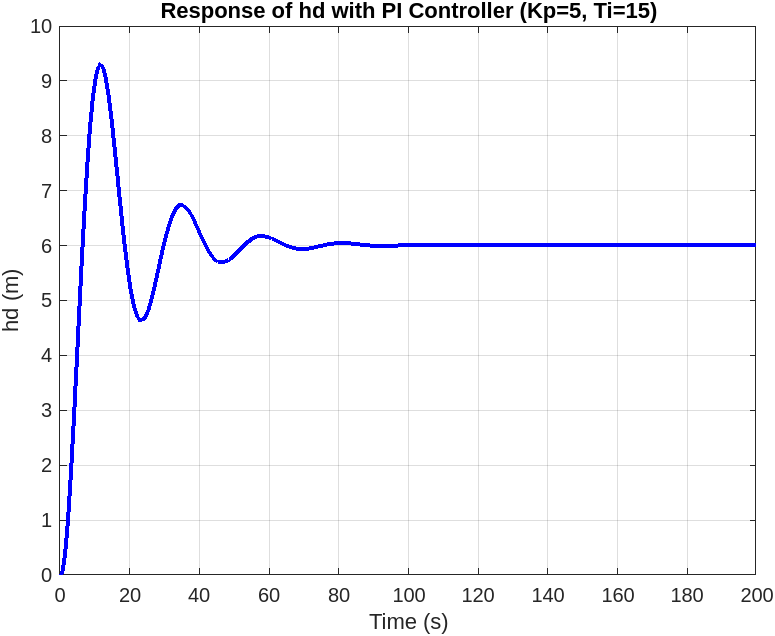
\includegraphics[width=\linewidth]{piController.png}
  \caption*{Figure 15: System Output with PI Controller}
\end{minipage}\hfill
\begin{minipage}{0.48\textwidth}
  \centering
  \includegraphics[width=\linewidth]{PIControllerSimulated.png}
  \caption*{Figure 16: ESS value and transient parameters values}
\end{minipage}
\end{figure}


\appendix
\chapter{Appendix}
\section{Code}
\begin{lstlisting}[language=Matlab, caption=project code,label=lst:code]
A1 = 5; A2 = 4; R1 = 3; R2 = 5;
% State-space matrices

% Assume our state is [h1, h2] , input is Qin, outputs are Q2, Q1, H1, H2

% State Matrix
A = [-1/(A1*R1), 1/(A1*R1);        % dh1/dt equation
    1/(A2*R1), -(1/(A2*R1) + 1/(A2*R2))];  % dh2/dt equation

% Input Matrix
B = [1/A1; 0];                     % Input only affects dh1/dt

% Output Matrix
C = [0, 1/R2;                      % q_out output
    1/R1, -1/R1;                  % q1 output
    1, 0;                         % h1 output
    0, 1];                        % h2 output

% Direct Feedthrough Matrix
D = zeros(4,1);

sys = ss(A,B,C,D,'InputName','Qin','OutputName',{'Q2','Q1','H1','H2'});

transfer_functions = {
    tf(sys(4)),  % H2/Qin
    tf(sys(3)),  % H1/Qin
    tf(sys(2)),  % Q1/Qin
    tf(sys(1))   % Q2/Qin
    };

names = {'H2(S)/Qin(S)', 'H1(S)/Qin(S)', 'Q1(S)/Qin(S)', 'Q2(S)/Qin(S)'};

for k = 1:length(transfer_functions)
    tf_current = transfer_functions{k};
    [num, den] = tfdata(tf_current, 'v');

    fprintf('\n\n\n%s = \n\n', names{k});

    % Print numerator
    for i = 1:length(num)
        power = length(num)-i;
        if num(i) == 0
            continue;
        end
        if power > 0
            if num(i) == 1
                fprintf('S^%d + ', power);
            else
                fprintf('%.4gS^%d + ', num(i), power);
            end
        else
            fprintf('%.4g', num(i));
        end
    end

    % Print denominator
    fprintf('\n------------------\n');
    for i = 1:length(den)
        power = length(den)-i;
        if den(i) == 0
            continue;
        end
        if power > 0
            if den(i) == 1
                fprintf('S^%d + ', power);
            else
                fprintf('%.4gS^%d + ', den(i), power);
            end
        else
            fprintf('%.4g', den(i));
        end
    end

end

% Stability analysis
P = pole(tf(sys(4)));
fprintf('\n\n\nPoles of H2/Qin: P0 = %.4f, P1 = %.4f\n', P(1), P(2));
is_stable = isstable(tf(sys(4)));
fprintf('Is stable: %d\n', is_stable);

figure;
pzmap(tf(sys(4)));
title('Pole-Zero Map of H2/Qin');
grid on;

% Simulate response to a step input (1 m^3/s)
t = linspace(0, 500, 10000);  % 10,000 samples over 500 seconds
u = ones(size(t));           % Step input of 1 m^3/s

[y, t_out, x] = lsim(sys, u, t);

% Plot h1
figure;
plot(t_out, y(:,3), 'b', 'LineWidth', 1.5);
grid on;
title('h1 (m)');
xlabel('Time (s)');
ylabel('h1');

% Plot h2
figure;
plot(t_out, y(:,4), 'r', 'LineWidth', 1.5);
grid on;
title('h2 (m)');
xlabel('Time (s)');
ylabel('h2');

% Plot Q1
figure;
plot(t_out, y(:,2), 'g', 'LineWidth', 1.5);
grid on;
title('Q1 (m^3/s)');
xlabel('Time (s)');
ylabel('Q1');

% Plot Q2
figure;
plot(t_out, y(:,1), 'm', 'LineWidth', 1.5);
grid on;
title('Q2 (m^3/s)');
xlabel('Time (s)');
ylabel('Q2');

% Calculate steady-state values
steady_state_values = y(end, :);
fprintf('\nSteady-state values:\n');
fprintf('h1 = %.4f m\n', steady_state_values(3));
fprintf('h2 = %.4f m\n', steady_state_values(4));
fprintf('Q1 = %.4f m^3/s\n', steady_state_values(2));
fprintf('Q2 = %.4f m^3/s\n', steady_state_values(1));

% Modify the system to have a feedback with a reference signal h_d
sys_cl = feedback(sys(4,:),1);

% Simulate response to a step input (h_d = 5 meters)
t = linspace(0,100,10000);  % 10,000 samples over 100 seconds

hd = 5 * ones(size(t));

[h2_response,t_out] = lsim(sys_cl,hd,t);

% Plot h2 response
figure;
plot(t_out, h2_response, 'r', 'LineWidth', 2);
grid on;
title('Response of h2 to desired level h_d = 5m');
xlabel('Time (s)');
ylabel('h2 (m)');

info = stepinfo(h2_response, t_out, 5);  % 5 is the desired final value

fprintf('Rise time: %.4f seconds\n', info.RiseTime);
fprintf('Peak time: %.4f seconds\n', info.PeakTime);
fprintf('Maximum overshoot: %.2f%%\n', info.Overshoot);
fprintf('Settling time: %.4f seconds\n', info.SettlingTime);

% Steady-state error
ess = abs(5 - h2_response(end));
fprintf('Steady-state error (ess): %.4f meters\n', ess);

% adding the controller to the system

Kp_values = [1, 10, 100];
hd = 5 * ones(size(t));  % Desired height

for i = 1:length(Kp_values)
    Kp = Kp_values(i);
    
    % Closed-loop transfer function with proportional controller
    sys_cl = feedback(Kp * tf(sys(4)), 1);
    
    % Simulate response
    [h2_response, t_out] = lsim(sys_cl, hd, t);
    
    % Plot response
    figure;
    plot(t_out, h2_response, 'LineWidth', 2);
    grid on;
    title(sprintf('hd Response with Kp = %d', Kp));
    xlabel('Time (s)');
    ylabel('hd (m)');
    
    % Step response characteristics
    info = stepinfo(h2_response, t_out, 5);  % Final value = 5
    ess = abs(5 - h2_response(end));         % Steady-state error
    
    fprintf('\n\n--- Kp = %d ---\n', Kp);
    fprintf('Rise Time: %.4f s\n', info.RiseTime);
    fprintf('Peak Time: %.4f s\n', info.PeakTime);
    fprintf('Overshoot: %.2f %%\n', info.Overshoot);
    fprintf('Settling Time: %.4f s\n', info.SettlingTime);
    fprintf('Steady-State Error: %.4f m\n', ess);
end



% Define PI controller parameters
Kp = 5;
Ti = 15;

% Define PI controller transfer function: C(s) = Kp * (1 + 1/(Ti*s))
s = tf('s');
C = Kp * (1 + 1/(Ti*s));  % Alternatively: C = (Kp*Ti*s + Kp)/(Ti*s)

% Get plant G(s) = H2(s)/Qin(s)
G = tf(sys(4));  % From Qin to h2

% Closed-loop system: feedback of C(s)*G(s)
sys_cl_PI = feedback(C * G, 1);

% Simulate step response to desired h_d = 5m
t = linspace(0, 200, 10000);
hd = 6 * ones(size(t));

[h2_PI, t_out] = lsim(sys_cl_PI, hd, t);

% Plot response
figure;
plot(t_out, h2_PI, 'b', 'LineWidth', 2);
grid on;
title('Response of hd with PI Controller (Kp=5, Ti=15)');
xlabel('Time (s)');
ylabel('hd (m)');

% Analyze response characteristics
info = stepinfo(h2_PI, t_out, 5);
ess = abs(6 - h2_PI(end));

fprintf('\n--- PI Controller Results (Kp = 5, Ti = 15) ---\n');
fprintf('Rise Time: %.4f s\n', info.RiseTime);
fprintf('Peak Time: %.4f s\n', info.PeakTime);
fprintf('Overshoot: %.2f %%\n', info.Overshoot);
fprintf('Settling Time: %.4f s\n', info.SettlingTime);
fprintf('Steady-State Error: %.4f m\n', ess);

\end{lstlisting}

\end{document}